\documentclass[a4paper]{article}

%% Language and font encodings
\usepackage[english]{babel}
\usepackage[utf8x]{inputenc}
\usepackage[T1]{fontenc}


%% Sets page size and margins
\usepackage[a4paper,top=3cm,bottom=2cm,left=3cm,right=3cm,marginparwidth=1.75cm]{geometry}

%% Useful packages
\usepackage{amsmath}
\usepackage{graphicx}
\usepackage{tikz,pgfplots}
\usepackage[colorinlistoftodos]{todonotes}
\usepackage[colorlinks=true, allcolors=blue]{hyperref}
\usepackage{amsfonts}
\usepackage{bbm}
\usepackage{dsfont}
\usepackage{cancel}
\usepackage{tikz,tkz-base,tkz-fct}
\newcommand{\prob}{\mathbb{P}}
\newtheorem{definicion}{Definición}
\newtheorem{teorema}{Teorema}
\newtheorem{ejemplo}{Ejemplo}
\DeclareMathOperator*{\argmax}{Arg\,max}
\newtheorem{lem}{Lemma}
\newtheorem{prop}{Proposici\'on}
\newtheorem{cor}{Corolario}
\newtheorem{dem}{Demostración}
\numberwithin{equation}{subsection}


%% Aquí se pueden definir nuevas abreviaturas para algunos comandos

\def\sen{{\rm sen\mspace{1.5mu}}}
\def\C{\mathbb C}
\def\R{\mathbb R}
\def\N{\mathbb N}
\def\Q{\mathbb Q}
\def\Z{\mathbb Z}
\def\V{\mathbb V}
\def\E{\mathbb E}
\def\to{\rightarrow}
\newcommand{\pb}{\mathbb{P}}



\newcommand{\ds}{\displaystyle}


%Para hacer normas en tex

\providecommand{\norm}[1]{\lVert#1\rVert}
\providecommand{\normm}[1]{\bigg\lVert#1\bigg\rVert}


%integrales bacanes
\usepackage{ esint }

%Para poner en negrita en modo matemático
\newcommand{\negri}{\boldsymbol}




\title{Simulación Estocástica}
\author{Clase 1}
\date{30 de julio de 2019}

\begin{document}
\maketitle

\section{Introduction}
\subsection{Notación.}
    \begin{itemize}
        \item $i.i.d.$: 'Independientes e idénticamente distribuídas'.
        \item $(E,d)$: Espacio métrico $E$, con métrica $d$.
        \item $\mathcal{B}(E)$: Conjunto de borelianos de $E$.
        \item $C_b (E) := \{f:E \rightarrow R \,| \text{ f es contínua y acotada}\}$
        \item $\mathcal{P}(E)$: Espacio de las medidas de probabilidades sobre $E$.
    \end{itemize}
\section{Convergencia en Ley}
Partiremos este capítulo enunciando uno de los teoremas más importante de la teoría de probabilidades, el teorema del límite central.

\begin{teorema}[Teorema Central del Límite.] Dadas $(X_n)_{n\in\N}$ variables aleatorias $i.i.d.$, con \newline$\mu = \E(X_1)$ y $\sigma^2 = Var(X_1)$, finitas. Para el promedio $n-esimo$:
\begin{equation}
    \Bar{X}_n = \frac{1}{n}\sum_{i=1}^{n}X_i
\end{equation}
Se define la variable aleatoria $Z_n$ como:
\begin{equation}
    Z_n = \frac{\Bar{X}_n - \mu}{\sigma / \sqrt{n}}
\end{equation}
Entonces $Z_n$ converge "EN LEY" a una variable normal estándar $\mathcal{N}(0,1)$ a medida que $n$ tiende a infinito.
\end{teorema}

Los resultados y usos que se desprenden de este teorema son bastante variados; desde el cálculo de probabilidades para una muestra aleatoria simple, estimación de parámetros, hasta nos premite el uso de test de hipótesis para distribuciones normales en ocaciones en que desconocemos por completo la distribución de los datos.\footnote{Todos estos usos están restringidos bajo aproximaciones.}\\ \newline
Y no es que sea raro encontrar este tipo de usos, puesto que el teorema no nos pide absolutamente nada con respecto al tipo de  distribución de las variables aleatorias, dando la posibilidad de que éstas sean contínuas, discretas o cualesquiera que se nos pudiesen ocurrir en diversos espacios de trabajo. Sin embargo el resultado es el mimso, convergencia a una distribución absolutamente contínua.\\ \newline
Si $Z_n$ puede tomar varias formas dada la colección de variables $(X_n)_{n\in\N}$, ¿por qué converge a una distribución contínua? Para responder esta pregunta introduciremos las nociones de \textit{convergencia débil de medida de probabilidad}.\newpage

\subsection{Convergencia débil sobre espacios métricos}

Para el conjunto de medidas de probabilidad sobre el espacio métrico $E$, es decir; $\mathcal{P}(E)$, definiremos la siguiente operación.\\ Para toda $\mu \in \mathcal{P}(E)$ y para toda $f: E\rightarrow \R$ función medible:
\begin{equation}
    \langle \mu , f\rangle = \int_{E} f d\mu
\end{equation}
\begin{definicion} Decimos que una sucesión $(\mu_n)_{n\in\N}$ de elementos de $\mathcal{P}(E)$ converge DEBILMENTE a $\mu\in \mathcal{P}(E)$ si:
\[\langle \mu_n ,f\rangle\, \xrightarrow{n\rightarrow\infty}\, \langle \mu,f\rangle \hspace{0.5cm}\forall\,f\in C_b(E)\]
En tal caso anotamos: $\mu_n \Rightarrow \mu$.
\end{definicion}

\begin{ejemplo}
    Tomemos el espacio métrico $E=\R$ con su métrica usual $d(x,y) = |x-y|$, y sea la sucesión de medidas de probabilidad $\mu_n = \delta_{\frac{1}{n}}$, donde $\delta_a$ representa la "Delta de Dirac" en el punto $a$:
    \[\delta_a(x) = \begin{cases} 
            +\infty & \text{si }x=a   \\ 
            0 & \text{si }x\neq a \end{cases}\]
    
    Veremos que esta distribución converge débilmente a la distribución $\delta_0$.\\ \newline
    En efecto, sea $f \in C_b(\R)$, tenemos que:
    \[\langle \mu_n ,f\rangle = \int_\R f(x) \mu_n (dx) = \int_\R f(x) \delta_{\frac{1}{n}}(x) dx = f(1/n)\]
    Puesto que la función $f$ es contínua en todo $\R$, entonces:
    \[f(1/n) \xrightarrow{n\rightarrow\infty}\,f(0) = \langle \mu,f\rangle \]
    Por lo tanto, $\mu_n \Rightarrow \mu$.
\end{ejemplo}
Dado que el argumento utilizado en el ejemplo se sostuvo fuertemente de la continuidad de la función $f$, en general se tendrá que para cada sucesión de reales $(x_n)_n$ que converja a un punto $\Bar{x}$, se tendrá la convergencia de las medidas de Dirac: $\delta_{x_n}\Rightarrow \delta_{\Bar{x}}$. Se puede demostrar que esto es una doble implicancia, es decir; la convergencia debil de las medidas de Dicar implican la convergencia en $\R$ de la sucesión de los puntos.\\ \newline
Para traducir el \textit{teorema Central del Límite} en conceptos de convergencia de medidas de probabilidad debemos asociar el concepto de \textit{variable aleatoria} en función de la medida de probabilidad asociada.\\
Recordemos que una variable aleatoria a valores en $E$ es una función $X:\Omega \rightarrow E$ medible, donde $(\Omega, \mathcal{F},\pb)$ es un espacio de probabilidad (este espacio se encuentra usualmente implícito en la mayoría de las definiciones y cálculos de probabilidades).\\ Su LEY o DISTRIBUCIÓN, denotada como $\mathcal{L}(X) \in \mathcal{P}(E)$, se definie como:
\begin{equation}
   \mathcal{L}(X)(A) := \pb(X^{-1}(A))\hspace{0.5cm}\forall\,A\in\mathcal{B}(E) 
\end{equation}

\begin{definicion} Una sucesión $(X_n)_{n\in\N}$ de variables aleatorias en $E$ se dice que converge EN LEY o EN DISTRIBUCIÓN a una variable aleatoria $X$ si $(\mathcal{L}(X_n))_{n\in\N}$ converge débilmente a $\mathcal{L}(X)$, es decir:
\[\E[f(X_n)] \xrightarrow{n\rightarrow\infty}\,\E[f(X)]\hspace{0.5cm}\forall\,f\in\,C_b\]
En este caso anotamos: $X_n\,\xrightarrow{\mathcal{L}}\,X$ o $X_n\,\xrightarrow{d}\,X$.
\end{definicion}
Notamos que esta definición es idéntica a la anterior pero expresada en términos de la esperanza de la función $f$ en vez de la integral de la función bajo la medida de probabilidad.
\newpage
\begin{ejemplo} Sea el espacio métrico $E=\R$ y una sucesión de variables aleatorias $i.i.d.$ $(X_n)_{n\in\N}$, tal que para cada natural $n$, la variable tiene una distribución uniforme en el intervalor $(-1/n, 1/n)$, es decir; $X_n \sim unif(-\frac{1}{n},\frac{1}{n})$ $\forall\,n\in\N$.
\begin{figure}
\centering
    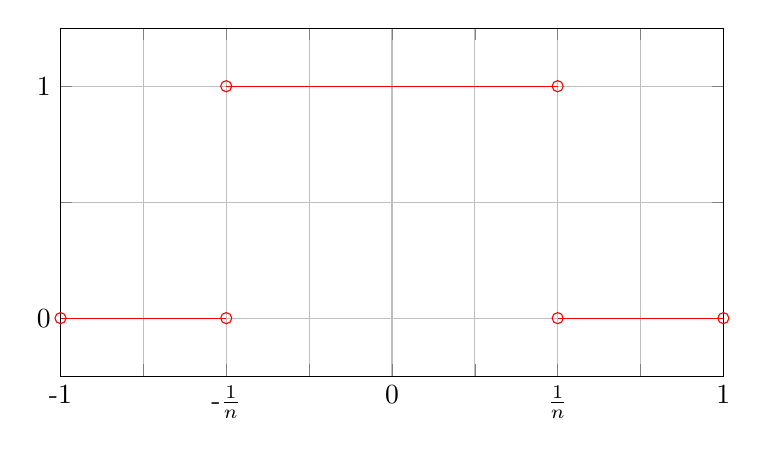
\begin{tikzpicture}
         \begin{axis}
        [width=10cm, height=6cm, xmin=-1, xmax=1, ymin=-0.25, ymax=1.25, xmajorgrids=true, ymajorgrids=true, xtick={-1,-0.75,-0.5,-0.25,0,0.25,0.5,0.75,1},  xticklabels={-1,,-$\frac{1}{n}$,,0,,$\frac{1}{n}$,,1}, ytick={0,0.5,1}, yticklabels={0,,1}]
        \addplot[color=red, mark=o] coordinates {(-1,0) (-0.5,0)};
        \addplot[color=red, mark=o] coordinates {(-0.5,1) (0.5,1)};
        \addplot[color=red, mark=o] coordinates {(0.5,0) (1,0)};
        \end{axis}
    \end{tikzpicture}
    \caption{Densidad uniforme $(-1/n$, $1/n)$.}
\end{figure}

Sea $f \in C_b(\R)$ una función contínua y acotada, entonces la esperanza $\E(f(X_n))$ está dada por:
\[\E(f(X_n)) = \int_{\R}f(x)\mu_n(dx)\]
Donde $\mu_n(dx)$ está dado por la densidad de la distribución de $X_n$, es decir la uniforme:\\ $\mu_n(dx) = \frac{n}{2} \mathbbm{1}_{(-\frac{1}{n},\frac{1}{n})}(x)dx$. Luego:
\[\E(f(X_n)) = \int_{\R}f(x)\,\frac{n}{2}\mathbbm{1}_{(-\frac{1}{n},\frac{1}{n})}(x)dx = \frac{n}{2}\int_{-\frac{1}{n}}^{\frac{1}{n}}f(x)dx\]
Haciendo uso del \textbf{teorema del valor medio} en integrales y de la continuidad de $f$, sabemos de la existencia de un valor $\xi_n \in (-\frac{1}{n},\frac{1}{n})$ tal que la integral anterior es de la forma:
\[\int_{-\frac{1}{n}}^{\frac{1}{n}}f(x)dx = \frac{2}{n}f(\xi_n)\]
Así,
\[\E(f(X_n)) = \frac{n}{2}\int_{-\frac{1}{n}}^{\frac{1}{n}}f(x)dx = f(\xi_n)\]
Por lo tanto la convergencia de $\E(f(X_n))$ estará dad por la convergencia de la nueva sucesión de puntos $(\xi_n)_{n\in\N}$. Para ver la convergencia de $\xi_n$ notemos que:
\begin{itemize}
    \item $\forall\,m\leq n$: $\left(-\frac{1}{n},\frac{1}{n}\right)\subset \left(-\frac{1}{m},\frac{1}{m}\right)$, por lo tanto:
    \[\xi_n \in \bigcap_{m=1}^{n}\left(-\frac{1}{m},\frac{1}{m}\right)\]
    Así la sucesión $\xi_n$ es acotada.
    \item Luego, la sucesión tiene al menos un punto de acumulación. Supongamos que $\Bar{\xi}$ es punto de acumulación de $(\xi_n)_n$, por lo dicho anteriormente debería suceder que:
    \[\Bar{\xi} \in \bigcap_{n\geq 1}\left(-\frac{1}{n},\frac{1}{n}\right) = \{0\}\]
    Finalmente se deduce que $\Bar{\xi}=0$.
\end{itemize}
Nuevamente, aplicando la continuidad de $f$:
\[\E(f(X_n)) = f(\xi_n) \rightarrow\,f(0) = \langle \delta_{0},f\rangle = \E(f(0))\]
\newpage
Así concluímos que:
\begin{itemize}
    \item $\mu_n \Rightarrow\,\delta_{0}$, donde $\mu_n$ estaba dada por las distribuciones uniformes.
    \item $X_n \xrightarrow{\mathcal{L}}\,X$, donde $X\equiv 0$.
\end{itemize}
\end{ejemplo}

\begin{ejemplo}
    Nuevamente tomamos como ejemplo $E=\R$, y definimos la siguiente medida:
    \[\mu_n = \frac{1}{n+1}\sum_{k=0}^{n}\delta_{k/n}\]
    De forma alternativa, definiendo $\mu_n = \mathcal{L}(X_n)$, donde $X_n$ corresponde al experimento de escoger un valor al azar del conjunto $\{0,\frac{1}{n},\frac{2}{n},\cdots,\frac{n}{n}\}$ y sea $\mu = \mathcal{L}(X)$, con $X\sim unif(0,1)$. Entonces $\forall$ $f\in C_b(\R)$:
    \[\langle \mu_n ,f\rangle = \frac{1}{n+1}\sum_{k=0}^{n} \langle \delta_{k/n},f\rangle = \frac{1}{n+1}\sum_{k=0}^{n}f(k/n)\]
    Notando que, para cada $n\in\N$ el conjunto $\{\frac{k}{n}\,|\,k=0,\cdots,n\}$ representa un refinamiento del intervalo $[0,1]$ y $f$ es una función acotada y contínua en ese intervalo (por lo tanto es \textit{Riemann-integrable}), entonces la suma anterior converge por ser suma de riemann, y:
    \[\langle \mu_n ,f\rangle = \frac{1}{n+1}\sum_{k=0}^{n}f(k/n) \xrightarrow{n\rightarrow\infty}\, \int_{0}^{1}f(x)dx = \langle \mu,f\rangle\]
    Luego $\mu_n \Rightarrow\,\mu$, i.e. $X_n \xrightarrow{\mathcal{L}}\,X$.
\end{ejemplo}
\subsubsection{El Teorema Portmanteau}
El siguiente teorema nos proporciona útiles equivalencias a la convergencia débil; cada una de ellas sirve como una definición. Un conjunto $A \in \mathcal{B}(E)$ cuya frontera $\partial A$ satisfaga que $\mu(\partial A) = 0$ se dirá conjunto \textit{$\mu$-contínuo} (Note que $\partial A$ es cerrado, por lo tanto pertenece a $\mathcal{B}(E)$).
\begin{teorema}[Portmanteau] Sean $\mu_n,\mu \in \mathcal{P}(E)$. Las siguientes propociciones son equivalentes:
\begin{itemize}
    \item[i)] $\mu_n \Rightarrow \mu$
    \item[ii)] $\langle \mu_n,f\rangle \rightarrow\, \langle \mu, f\rangle$ para toda función $f$ acotada y uniformemente contínua.
    \item[iii)] $\langle \mu_n , f \rangle \rightarrow\, \langle \mu, f\rangle$ para toda función $f$, Lipschitz.
    \item[iv)] $\limsup_n \mu_n(F) \leq \mu(F)$   $\forall F \subset E$ cerrado.
    \item[v)] $\liminf_n \mu_n(G) \geq \mu(G)$     $\forall G\subset E$ abierto.
    \item[vi)] $\lim\, \mu_n(A) = \mu(A)$ para todo $A$, conjunto \textit{$\mu$-contínuo}. 
\end{itemize}
\end{teorema}
Notemos que, en el caso del \textbf{Ejemplo 1}, la desigualdad del punto $iii)$ se satisface estrictamente si $F=\{0\}$, de la misma forma en el punto $iv)$ si $G=\{0\}^{c}$. Si tomamos $A=\{0\}$, la convergencia no se alcanza en el punto $vi)$, pero esto no contradice el teorema, ya que la medida límite de $\partial \{0\} = \{0\}$ es 1, no 0. 

\end{document}
